% VAE: networks output conditional-distribution parameters; an observation is
% scored during training and sampled from the decoder distribution at generation.
\documentclass[border=0pt]{standalone}
\usepackage{amsmath,amssymb}
% Shared visual language for the figures of the book.
% Every figure in this directory loads this file so the chapter reads as one system.
% NOTE: no blank lines are allowed inside \tikzset{...} (a blank line emits \par
% and breaks key scanning).
\NeedsTeXFormat{LaTeX2e}
\ProvidesPackage{figstyle}[2026/10/21 Figure style for Free Energy to LLMs]

\RequirePackage{tikz}
\usetikzlibrary{arrows.meta,positioning,calc,fit,shapes.geometric,shapes.misc,%
  backgrounds,matrix,decorations.pathreplacing,decorations.markings,patterns.meta}

% ---------------------------------------------------------------- palette
% Same values as book/preamble/style.tex, prefixed with F.
\definecolor{FNavy}{HTML}{14324A}
\definecolor{FTeal}{HTML}{0E7490}
\definecolor{FSky}{HTML}{E7F5F8}
\definecolor{FOrange}{HTML}{D97706}
\definecolor{FAmber}{HTML}{FFF3D6}
\definecolor{FInk}{HTML}{1F2937}
\definecolor{FSlate}{HTML}{64748B}
\definecolor{FMist}{HTML}{F5F7FA}
\definecolor{FRose}{HTML}{9F1239}
\definecolor{FRoseMist}{HTML}{FFF1F2}

% ---------------------------------------------------------------- semantics
% Teal   = probability / model / data object
% Orange = training objective, cost, or the quantity moved through the system
% Navy   = neutral structure
% Slate  = secondary label or metadata
% Rose   = failure mode, hazard, masked-out region
\tikzset{
  % Lay figures out in millimetres.  A figure designed 168mm wide is included at
  % \textwidth, so its fonts appear at exactly the size written here.
  every picture/.style={x=1mm,y=1mm,font=\small,line cap=round,line join=round},
  % ---- block styles
  nbase/.style={draw,rounded corners=1.2pt,align=center,inner sep=2.4pt,%
    minimum height=7mm,text=FInk},
  nteal/.style={nbase,draw=FTeal,fill=FSky},
  norange/.style={nbase,draw=FOrange,fill=FAmber},
  nnavy/.style={nbase,draw=FNavy,fill=white},
  nsoft/.style={nbase,draw=FSlate!55,fill=FMist},
  nrose/.style={nbase,draw=FRose,fill=FRoseMist},
  ghost/.style={draw=none,fill=none,align=center,inner sep=1pt},
  plain/.style={draw=none,fill=none,align=center,inner sep=0pt},
  % ---- arrows
  ar/.style={-{Latex[length=1.7mm,width=1.35mm]},draw=FSlate,line width=0.75pt},
  ard/.style={ar,dashed},
  arteal/.style={ar,draw=FTeal},
  arorange/.style={ar,draw=FOrange},
  arrose/.style={ar,draw=FRose},
  thickar/.style={ar,line width=1.2pt},
  % ---- text roles
  ftitle/.style={font=\large\bfseries,text=FNavy,align=center},
  ptitle/.style={font=\small\bfseries,text=FNavy,align=center},
  ptitleo/.style={font=\small\bfseries,text=FOrange,align=center},
  lbl/.style={font=\scriptsize,text=FSlate,align=center,inner sep=1pt},
  lblt/.style={lbl,text=FTeal},
  lblo/.style={lbl,text=FOrange},
  lbln/.style={lbl,text=FNavy},
  lblr/.style={lbl,text=FRose},
  sub/.style={font=\scriptsize,text=FSlate!90,align=center,inner sep=1pt},
  monob/.style={font=\ttfamily\scriptsize,text=FInk,inner sep=1pt},
  mathb/.style={font=\small,text=FInk,inner sep=1pt},
  eqn/.style={font=\scriptsize,inner sep=1.5pt,text=FInk},
  % ---- decorations
  brace/.style={decorate,decoration={brace,amplitude=2.4pt},draw=FSlate,%
    line width=0.6pt},
  bracet/.style={brace,draw=FTeal},
  braceo/.style={brace,draw=FOrange},
  axis/.style={draw=FSlate!55,line width=0.6pt},
  guide/.style={draw=FSlate!45,line width=0.5pt,dashed},
  halolabel/.style={font=\scriptsize,text=FInk,fill=white,fill opacity=0.85,%
    text opacity=1,inner sep=1.4pt,align=center},
}

% Figure title above the drawing, anchored at the figure's top-left.
\newcommand{\figtitle}[2][0]{%
  \node[ftitle,anchor=north west,outer sep=0pt] at (#1,0) {#2};}

% Rounded panel behind a subgroup of nodes.
\newcommand{\figpanel}[3][]{%
  \node[draw=FSlate!35,fill=#3,rounded corners=2pt,inner sep=2.6mm,#1] {#2};}

\endinput

\begin{document}
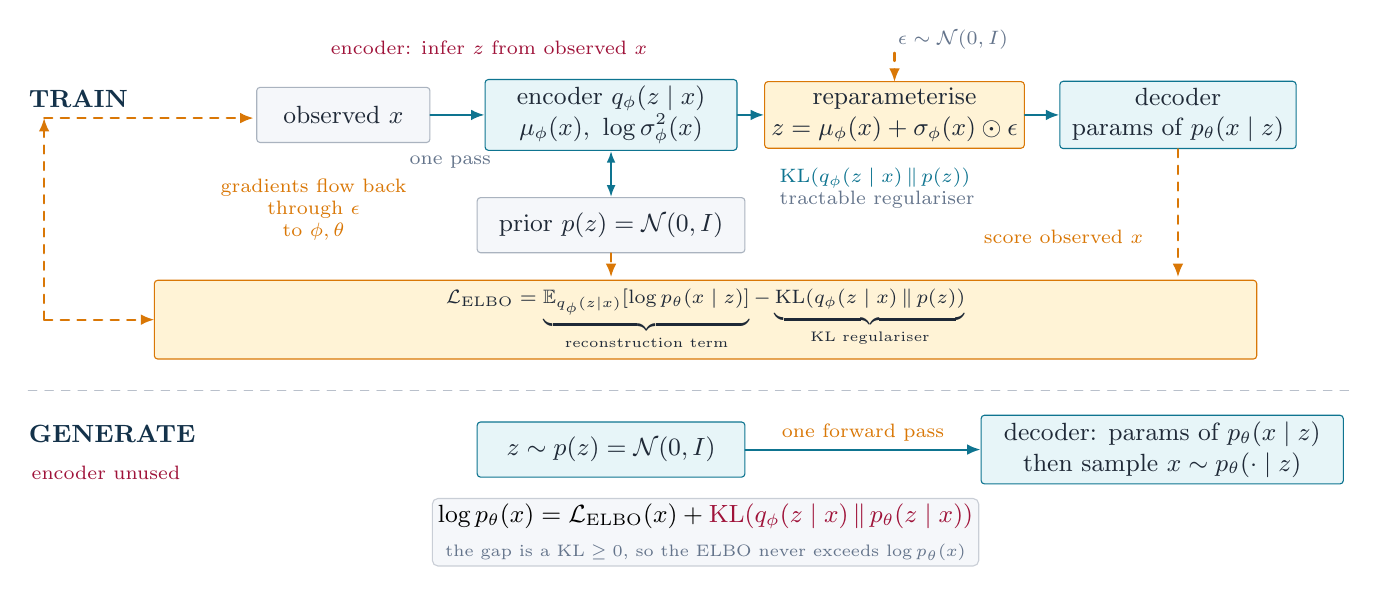
\begin{tikzpicture}
\node[lblr,anchor=west] at (38,62.5) {encoder: infer $z$ from observed $x$};
\node[lbl,anchor=west] at (110,63.5) {$\epsilon\sim\mathcal N(0,I)$};
\draw[arorange,dashed] (110,61.9) -- (110,58.2);
\node[plain,anchor=west,font=\small\bfseries,text=FNavy] at (0,56) {TRAIN};
\node[nsoft,minimum width=22mm] (data) at (40,54) {observed $x$};
\node[nteal,minimum width=32mm] (enc) at (74,54) {encoder $q_\phi(z\mid x)$\\$\mu_\phi(x),\ \log\sigma_\phi^2(x)$};
\node[norange,minimum width=32mm] (rep) at (110,54) {reparameterise\\$z=\mu_\phi(x)+\sigma_\phi(x)\odot\epsilon$};
\node[nteal,minimum width=30mm] (dec) at (146,54) {decoder\\params of $p_\theta(x\mid z)$};
\draw[arteal] (data)--(enc);
\draw[arteal] (enc)--(rep);
\draw[arteal] (rep)--(dec);
\node[lbl,anchor=north west] at (48,49.2) {one pass};
\node[nsoft,minimum width=34mm] (prior) at (74,40) {prior $p(z)=\mathcal N(0,I)$};
\draw[arteal,{Latex[length=1.5mm]}-{Latex[length=1.5mm]}] (enc.south) -- (prior.north);
\node[lblt,anchor=west] at (95,46) {$\mathrm{KL}(q_\phi(z\mid x)\,\Vert\,p(z))$};
\node[lbl,anchor=west] at (95,43.2) {tractable regulariser};
\node[norange,minimum width=140mm,minimum height=10mm,font=\scriptsize] (elbo) at (86,28)
  {$\mathcal L_{\mathrm{ELBO}}=\underbrace{\mathbb{E}_{q_\phi(z\mid x)}[\log p_\theta(x\mid z)]}_{\text{reconstruction term}}-\underbrace{\mathrm{KL}(q_\phi(z\mid x)\,\Vert\,p(z))}_{\text{KL regulariser}}$};
\draw[arorange,dashed] (prior.south) -- (74,33.4);
\draw[arorange,dashed] (dec.south) -- (146,33.4);
\node[lblo,anchor=east] at (142,38.5) {score observed $x$};
\draw[arorange,dashed] (2,28) -- (16,28);
\draw[arorange,dashed] (2,28) -- (2,53.6);
\draw[arorange,dashed] (2,53.6) -- (28.6,53.6);
\node[lblo,anchor=west] at (24,42) {gradients flow back\\through $\epsilon$\\to $\phi,\theta$};
\draw[guide] (0,19) -- (168,19);
\node[plain,anchor=west,font=\small\bfseries,text=FNavy] at (0,13.5) {GENERATE};
\node[lblr,anchor=west] at (0,8.5) {encoder unused};
\node[nteal,minimum width=34mm] (z) at (74,11.5) {$z\sim p(z)=\mathcal N(0,I)$};
\node[nteal,minimum width=46mm] (dec2) at (144,11.5) {decoder: params of $p_\theta(x\mid z)$\\then sample $x\sim p_\theta(\cdot\mid z)$};
\draw[arteal] (z)--(dec2) node[midway,above=0.6mm,lblo] {one forward pass};
\node[draw=FSlate!35,fill=FMist,rounded corners=2pt,inner sep=2pt,align=center] at (86,1)
  {$\log p_\theta(x)=\mathcal L_{\mathrm{ELBO}}(x)+\textcolor{FRose}{\mathrm{KL}(q_\phi(z\mid x)\,\Vert\,p_\theta(z\mid x))}$\\[0.4mm]
   {\fontsize{6}{7}\selectfont\color{FSlate}the gap is a $\mathrm{KL}\geq0$, so the ELBO never exceeds $\log p_\theta(x)$}};
\end{tikzpicture}
\end{document}
